% Mirror: https://github.com/SIGma-UIUC/presentation-format
% --------------------------------------------------------------------
% This is a simple Beamer document that uses beamerthemesigma.sty
% Reading the comments should help you create a presentation even if
% you've never used Beamer before.
% --------------------------------------------------------------------

% Set our document class to Beamer
\documentclass[aspectratio=169]{beamer}
% \documentclass[aspectratio=169, handout]{beamer}
% Add handout option to ignore pauses

% From Jeff E
\usepackage{algo}
% Some more macros
\usepackage{sigmastyle}


% Set a title
\title{Believe It or Not, Another Semester}

% Set a subtitle if you desire
\subtitle{}

% Whoever worked on the presentation:
\author{SIGma}

% Date looks ugly, so leave blank
\date{}

% An institute name, if you're so inclined
% \institute{University of Illinois Urbana-Champaign}

% Use the SIGma theme for this Beamer presentation
\usetheme{sigma}
% --------------------------------------------------------------------

% Begin document
\begin{document}

% Beamer calls each slide a "frame", defined within the environment:
% \begin{frame}
%   <frame content here>
% \end{frame}

% This frame is just the title.
\begin{frame}
\titlepage
\end{frame}

% A frame with the table of contents.
% This frame's title is "Outline".
\begin{frame}{Outline}
  \tableofcontents
\end{frame}

\begin{frame}{Updates!}
  % Let's put some real content in this frame:
  Weekly updates:
  \begin{itemize}
    \item We're back!
    \item \texttt{\#research-advice} in Discord
    \item \texttt{\#seminars} in Discord
    \item Come make meetings 
  \end{itemize}
\end{frame}

\section{Admins in No Particular Order}
\frame{\sectionpage}

\begin{frame}{Sam}
    \begin{itemize}
    \item CS PhD
    \item Doing Computational Geometry with Sariel Har-Peled
    \item SIGPwny
    \end{itemize}
\end{frame}

\begin{frame}{Hassam}
    \begin{itemize}
        \item CS Major (takes math classes for fun ???)
        \item SIGPwny Crypto Gang + Admin team + Infra lead
        \item CA for CS 341, CS 173
        \item Compiler research (paper accepted ASPLOS '24 !!!)
        \item Graduating (and subsequently selling out) this semester
    \end{itemize}
\end{frame}

\begin{frame}{Ryan}
    \begin{itemize}
    \item Not selling out yet - currently a junior in CS
    \item CA for CS\{222, 374, 461\}
    \item Interest in algorithmic game theory and fair division, currently working on approximation algorithms for division
    \item Attempting to do hardware
    \end{itemize} 
\end{frame}

\begin{frame}{Alex}
    \begin{itemize}
    \item Stats\&CS, Math Double Major
    \item Part of PeopleWeave Research Project
    \item CA for CS 225, CS 374
    \item Foosball Pro
    \end{itemize} 
\end{frame}

\begin{frame}{Porter}
    \begin{itemize}
    \item CS Major, Math Minor
    \item Intern at CDK Global over the summer
    \item CA for CS 128H
    \item Foosball Pro
    \end{itemize} 
\end{frame}

\begin{frame}{Anakin} 
        \begin{itemize}
        \item Doing research in ICLUE with Alexander Yong
        \item Did Computational Group Theory at an REU
        \item Used to do Graph Theory / Optimization Research with Sam
        \item SIGPwny Crypto\footnotemark\ Gang + Admin team
        \item Coffee Club
        \item CA for CS 173 + CS 225H, former 374 + 475
    \end{itemize}
    \footnotetext[1]{Not that one, the other one}
\end{frame}

\begin{frame}{Come Make Meetings!}
    Brand New: \emph{Short and Sweet Presentations} \pause
    \begin{itemize}
        \item 3 presentations each day
        \item 10-15 minutes long (\emph{Short})
        \item Probably some food and drink (\emph{Sweet})
        \item March 18th \& April 22nd
        \item Good way to show you are interested in being a future admin
    \end{itemize} \pause
    Join Discord + DM any @admin if interested
\end{frame}

\section{P vs NP}
\frame{\sectionpage}

% Might find a way to cut down to four slides, not 5

\begin{frame}{Complexity Classes}
    \begin{itemize}
        \item \emph{Complexity Classes} are groups of problems that are characterized by being of the same ``difficulty'' \pause
        \item ``Difficulty'' refers to big-$O$ notation: If an algorithm runs in $O(n^2)$ time, that means as the input size $n$ tends to infinity, the algorithm takes $cn^2$ time for some constant $c$ \pause
        \item Most people think about two classes: 
        \begin{itemize}
            \item problems with polynomial time algorithms
            \item problems requiring larger-than-polynomial time algorithms
        \end{itemize}
        % \item Complexity classes depend on three piece of information: \pause
        % \begin{enumerate}
        %     \item The types of input and output
        %     \item A computational model (Turing Machines, DFAs, etc)
        %     \item The level of difficulty
        % \end{enumerate}
    \end{itemize}
\end{frame}

\begin{frame}{Decision Problems}
   \begin{itemize}
       \item These are problems that have \emph{yes or no} answers \pause
       \item Examples:
       \begin{itemize}
           \item Is this list sorted?
           \item Does this graph have a path visiting every node exactly once (Hamiltonian path)?
           \item Is this number prime?
       \end{itemize}
       % \item Non-examples:
       % \begin{itemize}
       %     \item Sort this list.
       %     \item How many Hamiltonian paths are in this graph?
       %     \item What is the prime factorization of this number?
       % \end{itemize}
   \end{itemize} 
\end{frame}

\begin{frame}{Decision Problems}
    \begin{itemize}
        \item The typical computation model is a Turing Machine
        \begin{itemize}
            \item For all intents and purposes, a normal computer $+$ your favorite programming language\footnote{Unless your favorite language is HTML}
        \end{itemize} \pause
        \item The input size of the problem is usually part of the problem specification 
         \begin{itemize}
           \item Is this list of length $n$ sorted?
           \item Does this graph with $n$ nodes have a Hamiltonian path?
           \item Is this $n$-bit binary number prime?
       \end{itemize} 
    \end{itemize}
\end{frame}

\begin{frame}{Solving vs Verifying}
    \begin{itemize}
        \item For decision problems, the two big paradigms are \emph{solving} the problem and \emph{verifying} a solution \pause
        \item Consider the problem of finding a Hamiltonian path in a graph with $n$ nodes:
        \begin{itemize}
            \item \emph{solving}: Try all $n!$ orderings of nodes, see if any of them are a Hamiltonian path. Runs in $O(n * n!)$ time \pause
            \item \emph{verifying:} Given a candidate path, check if it is a Hamiltonian path. Runs in $O(n)$ time 
        \end{itemize}
    \end{itemize}
\end{frame}

\begin{frame}{The Million Dollar Question}
    \begin{itemize}
        \item In the year 2000, the Clay Mathematics Institute posed 7 Prize Problems where the people who found the solutions would get \$1,000,000
        \item The P vs NP problem is about whether or not the following two complexity classes are equal: \pause
        \begin{itemize}
            \item P: The set of decision problems with polynomial time algorithms to \emph{solve} the problem
            \item NP: The set of decision problems with polynomial time algorithms to \emph{verify} a solution
        \end{itemize}
    \end{itemize}
\end{frame}

\section{Circuits Like You've Never Seen Before}
\frame{\sectionpage}

\begin{frame}{A New (Old) Approach to P vs NP}
    \begin{itemize}
        \item One of the most influencial papers in complexity theory is ``Completeness classes in algebra'' by Valient \cite{vp-vnp}
        \item He proposed an \emph{algebraic} approach to the P vs NP problem 
        \item This has been furthered by Mulmuley and Sohini and is currently seen as the most viable approach to resolving P vs NP \pause
        \item \emph{Idea:} Polynomials are our computational model
    \end{itemize}
\end{frame}

\begin{frame}{Algebraic Circuits}
    \[
        x^4 - 4 x^3 + 2 x^2 + 4 x - 3 = (x - 1)^2(x + 1)(x - 3)
    \]
    \begin{minipage}[t]{0.49\textwidth}
        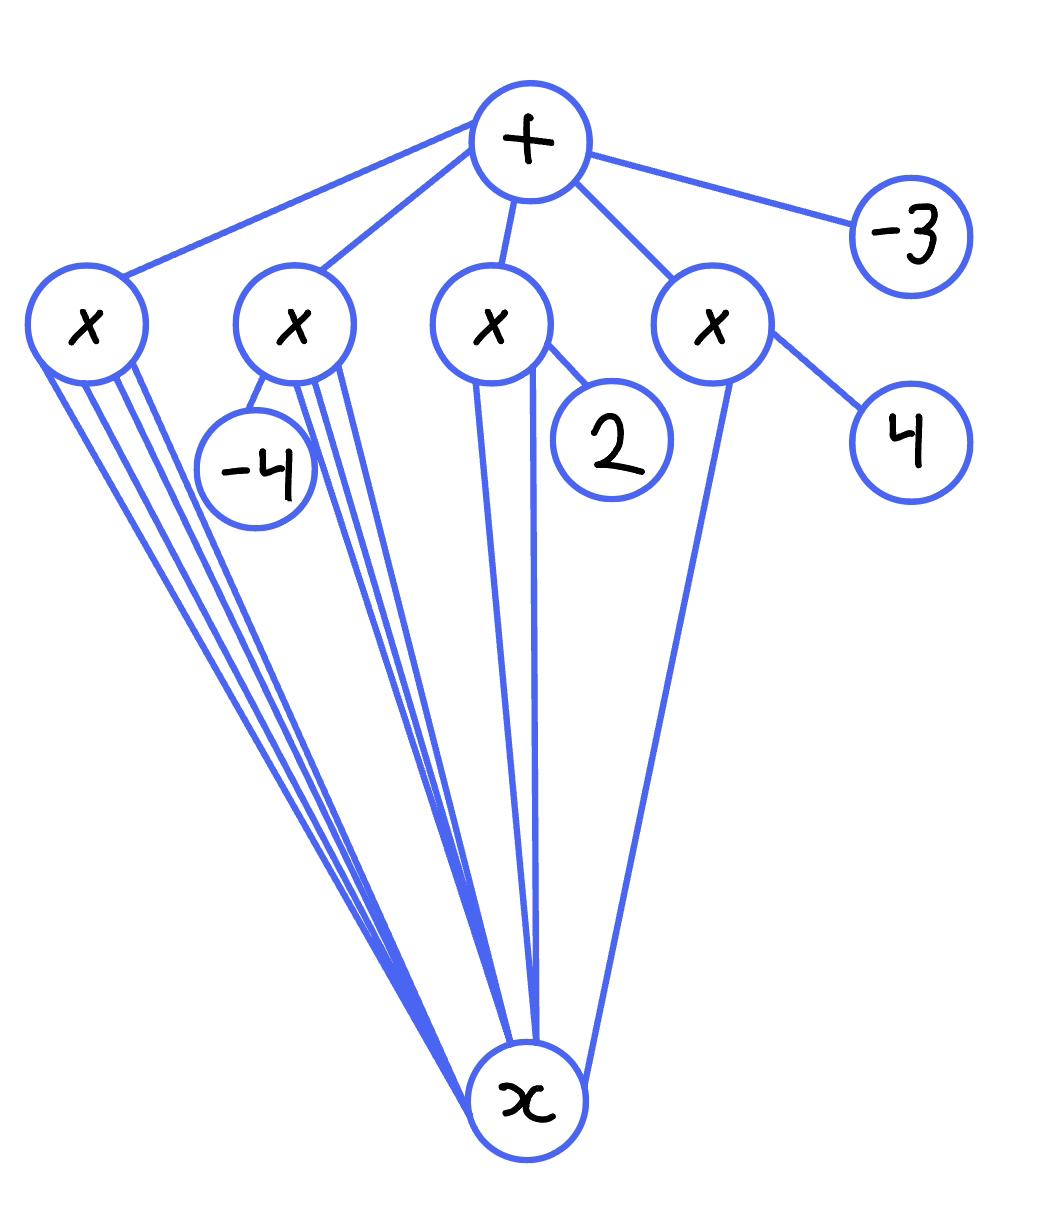
\includegraphics[width=0.875\textwidth]{unfac.jpeg}
    \end{minipage}\pause
    \begin{minipage}[t]{0.49\textwidth}
        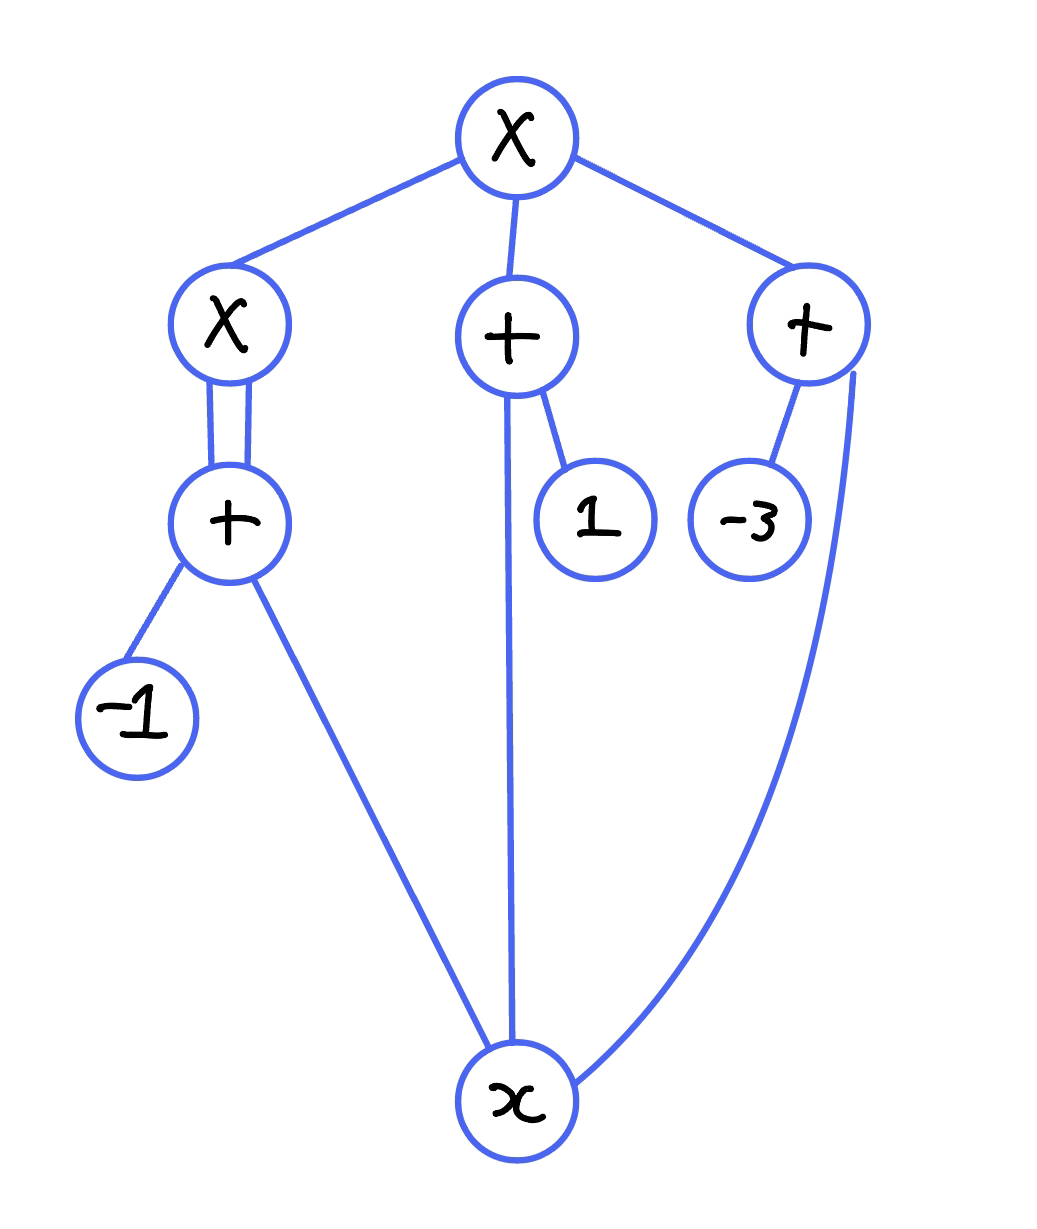
\includegraphics[width=0.875\textwidth]{fac.jpeg}
    \end{minipage}
\end{frame}

\begin{frame}{Complexity}
    \begin{itemize}
        \item There are two main measures of complexity of an algebraic circuit: \pause
        \begin{itemize} 
            \item \emph{Size:} Number of nodes \pause
            \item \emph{Depth:} Length of the longest path from an input to the output gate \pause
        \end{itemize}
        \item Given a polynomial $f$, we can ask two types of questions: \pause
        \begin{itemize}
            \item Can we construct a circuit for $f$ of small \{size/depth\}? \pause
            \item Can we show no such small circuit for $f$ exists?
        \end{itemize}
    \end{itemize}
\end{frame}

\begin{frame}{Complexity}
    Recall the normal computational model for a problem with input size $n$:
    \begin{itemize}
        \item P: Decision problems we can \emph{solve} in $\poly(n)$ time.
        \item NP: Decision problems whose solution we can \emph{verify} in $\poly(n)$ time.
        \item P $\subseteq$ NP
        \item \textcolor{sigma@alertred}{P $\subsetneq$ NP}: Million Dollar Question
    \end{itemize} \pause
    Now consider a polynomial $f$ of degree $d$. We define \emph{Valient's P / NP}: \pause
    \begin{itemize}
        \item VP: $f$ has a $\poly(d)$ size circuit to \emph{compute it}\pause
        \item VNP: Given some monomial, we can \emph{find the coefficient} of the monomial in $f$ with a $\poly(d)$ size circuit \pause
        \item VP $\subseteq$ VNP
    \end{itemize}
\end{frame}

\begin{frame}{A Tale of Two Polynomials}
        \vspace{-15pt}
    Consider an $n \times n$ matrix $X$ with entries $x_{i, j}$
    \begin{align*}
        \det(X) = \sum_{i = 1}^n (-1)^i \cdot x_{1, i} \cdot \det(X_{-1, -i}) && \perm(X) = \sum_{i = 1}^n x_{1, i} \cdot \perm(X_{-1, -i}) 
    \end{align*} \pause
    \vspace{-15pt}
    \begin{itemize}
        \item $\det(X) \in$ VP: Gaussian Elimination gives $O(n^3)$ size \pause
        \item $\det(X) \in$ VNP: VP $\subseteq$ VNP \pause
        \item $\perm(X) \in$ VNP: Just trust me \pause
        \item \textcolor{sigma@alertred}{$\perm(X) \notin$ VP}: Algebraic Million Dollar Question
    \end{itemize}
    \mbox{If VP = VNP and the (generalized) Riemann Hypothesis holds, then ``P = NP''}
    \cite{burg}
\end{frame}

\section{Matchings in Parallel}
\frame{\sectionpage}

\begin{frame}{A Match Made in Heaven}
    \begin{minipage}[t]{0.49\textwidth}
        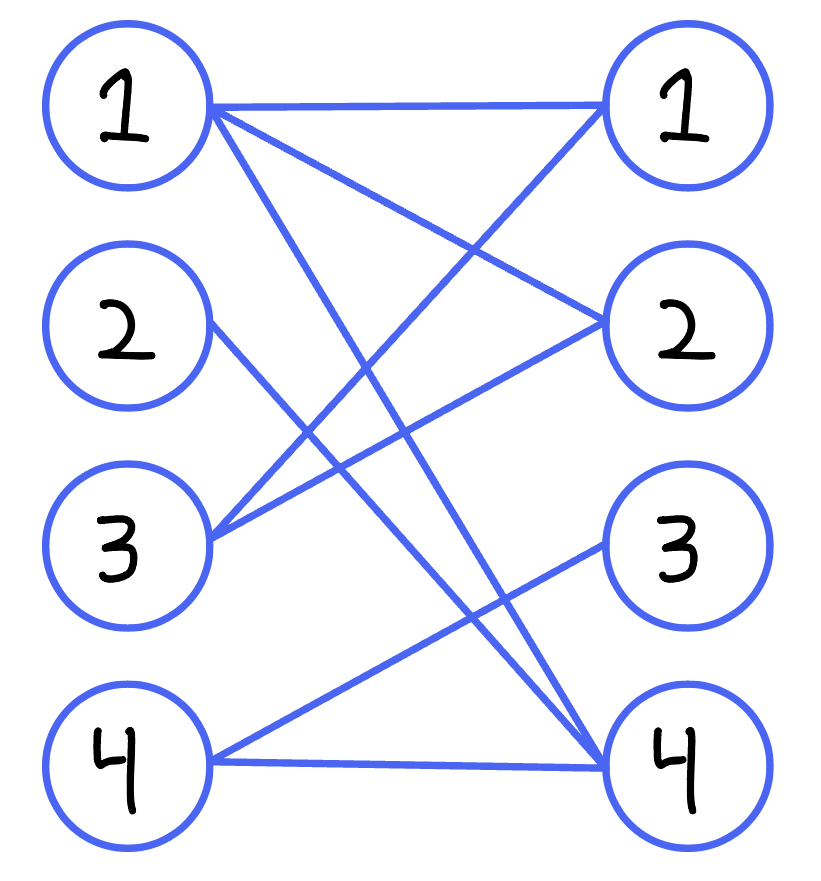
\includegraphics[width=0.875\textwidth]{G.png}
    \end{minipage}\pause
    \begin{minipage}[t]{0.49\textwidth}
        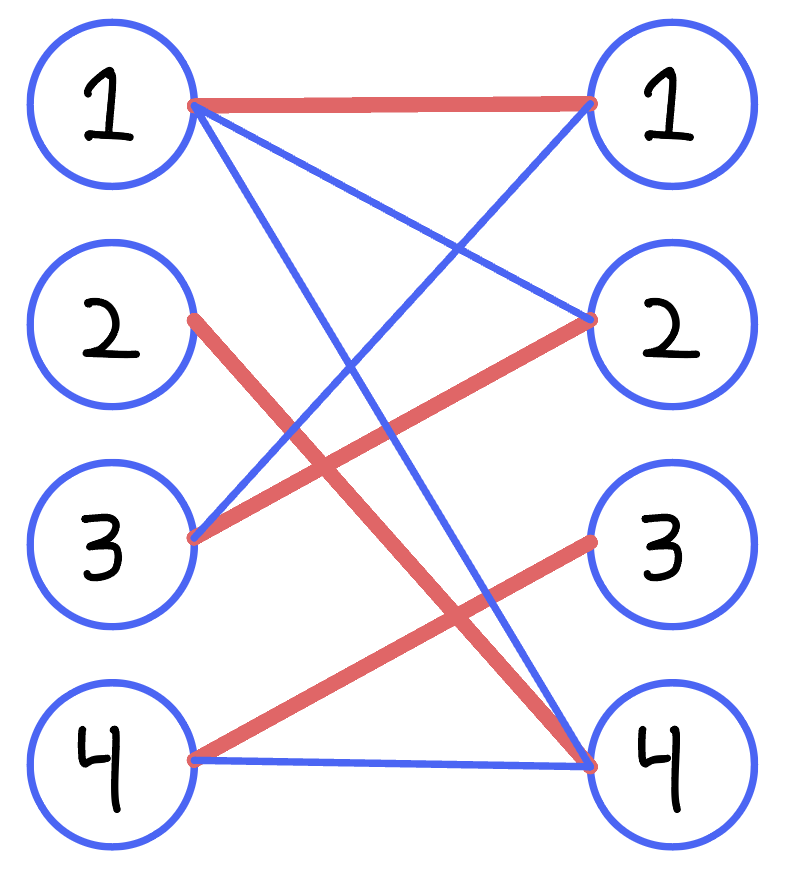
\includegraphics[width=0.875\textwidth]{M.png}
    \end{minipage}
\end{frame}

\begin{frame}{Algebraic Computation}
    \begin{itemize}
        \item Determining if there is a perfect matching in a bipartite graph can be determined in polynomial time \pause
        \item We will see how to do this with an algorithm that can be \emph{parallelized}
    \end{itemize}
\end{frame}

\begin{frame}{Turning a Graph into a Polynomial}
    Given a graph $G = (V, E)$ with $n$ vertices labeled $1, \ldots, n$, let $X$ be a matrix such that 
    \[
        X_{i, j} = \begin{cases}
                        x_{i, j} & \text{if } i \tofrom j \in E \\
                        0        & \text{if } i \tofrom j \notin E \\
                    \end{cases}
    \]
    \begin{minipage}{0.45\textwidth}
        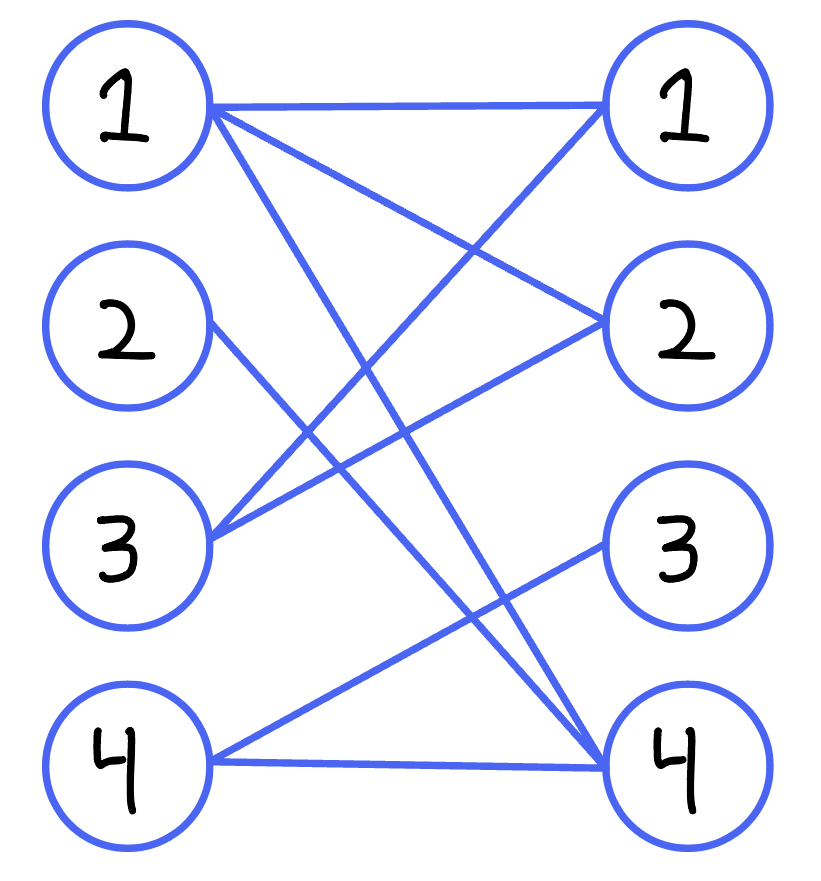
\includegraphics[width=0.75\textwidth]{G.png}
    \end{minipage}\hfill
    \begin{minipage}{0.45\textwidth}
        $$
            \begin{pmatrix}
                x_{1, 1} & x_{1, 2} &    0     & x_{1, 4} \\
                    0    &    0     &    0     & x_{2, 4} \\
                x_{3, 1} & x_{3, 2} &    0     &    0     \\
                    0    &    0     & x_{4, 3} & x_{4, 4} 
            \end{pmatrix}
        $$
    \end{minipage}
\end{frame}

\begin{frame}{Alternate Formulation}
    Consider an $n \times n$ matrix $X$ with entries $x_{i, j}$
    \begin{align*}
        \det(X) = \sum_{i = 1}^n (-1)^i \cdot x_{1, i} \cdot \det(X_{-1, -i}) && \perm(X) = \sum_{i = 1}^n x_{1, i} \cdot \perm(X_{-1, -i}) 
    \end{align*} \pause
    \vspace{-10pt}
    \begin{align*}
        \det(X) = \sum_{\sigma \in S_n} \sgn(\sigma) x_{1, \sigma(1)} \cdots x_{n, \sigma(n)} && \perm(X) = \sum_{\sigma \in S_n} x_{1, \sigma(1)} \cdots x_{n, \sigma(n)}
    \end{align*}
    \vspace{-10pt}
    \begin{itemize}
        \item $S_n = $ set of all orderings of integers $1, \ldots, n$ \pause
        \item An \emph{inversion} in $\sigma$ is if $i < j$ and $\sigma(i) > \sigma(j)$ 
        \item
        \[
            \sgn(\sigma) = \begin{cases}
                                1 & \text{if number of inversions in } \sigma \text{ is even} \\
                                -1 & \text{if number of inversions in } \sigma \text{ is odd}
                            \end{cases}
        \]
        % \item $\sgn(\sigma) = $
        % \begin{itemize}
        %     \item 1 if number of inversions in $\sigma$ is even
        %     \item -1 if number of inversions in $\sigma$ is odd
        % \end{itemize}
    \end{itemize}
\end{frame}

\begin{frame}{The Final Algorithm}
    \begin{itemize}
        \item Let $X$ be the matrix from before constructed from $G$
        \item \emph{Claim:} $\det(X) \neq 0 \iff G$ has a perfect matching \pause
        \begin{itemize}
            \item \emph{Proof:} Think about which orderings $\sigma$ correspond to matchings
        \end{itemize}
        \item Recall that a non-zero degree $d$ polynomial has at most $d$ zeroes
        \item $\det(X)$ has degree $\leq n^2$
    \end{itemize} \pause
    \begin{nalgo}
        \underline{\textsc{Match}($G$)}\+
    \\      $X \gets$ matrix constructed from $G$
    \\      $f(\overline{x}) \gets \det(X)$ 
    \\      $P \sample n^2 + 1$ distinct random points from $\R^{n^2}$
    \\      for $\overline{p} \in P$:\+
    \\          if $f(\overline{p}) \neq 0$:\+
    \\              return \true\-\-
    \\      return \false
    \end{nalgo}
\end{frame}

% Asking questions is fun but we should answer some first
\begin{frame}{}
      \begin{center}
    {\color{sigma@mainblue} \LARGE Questions?}
  \end{center}
\end{frame}

% Quotes are fun, find some to use!
\font\eightss=cmssq8
\font\eightssi=cmssqi8
\newcommand\quoteAuthorDate[2]{\begingroup
  \baselineskip 10pt
  \parfillskip 0pt
  \interlinepenalty 10000 % not needed in example
  \leftskip 0pt plus 40pc minus \parindent
  \let\rm=\eightss
  \let\sl=\eightssi
  \everypar{\sl}#1\par
  \nobreak\smallskip
  \noindent\rm--- #2\unskip\enspace\par
  \endgroup}
% If someone can figure out how to horizontally center this and make the text bigger that'd be cool
\begin{frame}
    \begin{center}
        \item \quoteAuthorDate{Algorithms are for people who don't know how to buy RAM}{Clay Shirky}{\color{sigma@mainblue}}
    \end{center}
\end{frame}

% Remove this slide if you came up with all the material yourself
\begin{frame}[allowframebreaks]{Bibliography}
    \tiny
    \bibliography{refs}
    \bibliographystyle{alpha}
\end{frame}

\end{document}